%-----------------------------------------------------------------------
% Template File for Science China Information Sciences
% Downloaded from http://scis.scichina.com
% Please compile the tex file using LATEX or PDF-LATEX or CCT-LATEX
%-----------------------------------------------------------------------

\documentclass{SCIS2026}
%%%%%%%%%%%%%%%%%%%%%%%%%%%%%%%%%%%%%%%%%%%%%%%%%%%%%%%
%%% Author's definitions for this manuscript
%%% 作者附加的定义
%%% 常用环境已经加载好, 不需要重复加载
%%%%%%%%%%%%%%%%%%%%%%%%%%%%%%%%%%%%%%%%%%%%%%%%%%%%%%%

\usepackage{cleveref}
\crefname{figure}{Fig.}{Figs.}

\crefformat{theorem}{Theorem~#2#1#3}
\crefrangeformat{theorem}{Theorems~#3#1#4-#5#2#6}
\crefmultiformat{theorem}{Theorems~#2#1#3}{ and ~#2#1#3}{, ~#2#1#3}{ and ~#2#1#3}

\crefformat{assumption}{Assumption~#2#1#3}
\crefrangeformat{assumption}{Assumptions~#3#1#4-#5#2#6}
\crefmultiformat{assumption}{Assumptions~#2#1#3}{ and ~#2#1#3}{, ~#2#1#3}{ and ~#2#1#3}

\crefformat{lemma}{Lemma~#2#1#3}
\crefrangeformat{lemma}{Lemmas~#3#1#4-#5#2#6}
\crefmultiformat{lemma}{Lemmas~#2#1#3}{ and ~#2#1#3}{, ~#2#1#3}{ and ~#2#1#3}

\crefformat{section}{Section~#2#1#3}
\crefrangeformat{section}{Sections~#3#1#4-#5#2#6}
\crefmultiformat{section}{Sections~#2#1#3}{ and ~#2#1#3}{, ~#2#1#3}{ and ~#2#1#3}

\newcommand{\kk}{^{(k)}}
\newcommand{\dd}{\mathrm{diag}}
\newcommand{\ml}{\mathcal{L}}
\newcommand{\tp}{^\top}
\newcommand{\ik}{_{k=1}^{K}}
\newcommand{\inn}{_{i=1}^{N}}
\newcommand{\md}{\mathrm{d}}

%%%%%%%%%%%%%%%%%%%%%%%%%%%%%%%%%%%%%%%%%%%%%%%%%%%%%%%
%%% Begin. 开始
%%%%%%%%%%%%%%%%%%%%%%%%%%%%%%%%%%%%%%%%%%%%%%%%%%%%%%%
\begin{document}
%\oa
%%%%%%%%%%%%%%%%%%%%%%%%%%%%%%%%%%%%%%%%%%%%%%%%%%%%%%%
%%% Authors do not modify the information below
%%% 作者不需要修改此处信息
\ArticleType{RESEARCH PAPER}
%\SpecialTopic{}
\Year{2025}
\Month{January}
\Vol{68}
\No{1}
\DOI{}
\ArtNo{}
\ReceiveDate{}
\ReviseDate{}
\AcceptDate{}
\OnlineDate{}
\AuthorMark{}
\AuthorCitation{}
%%%%%%%%%%%%%%%%%%%%%%%%%%%%%%%%%%%%%%%%%%%%%%%%%%%%%%%

%%% title: 标题
%%%   \title{title}{title for citation}
\title{Turing patterns on multiplex-networked activator-inhibitor systems with multiplicative noise}{Dai H, Wen G, Chen G, et al. Turing patterns on multiplex-networked activator-inhibitor systems with multiplicative noise}

%%% Corresponding author: 通信作者
%%%   \author[number]{Full name}{{email@xxx.com}}
%%% General author: 一般作者
%%%   \author[number]{Full name}{}
%%% Equal Contribution: 同等贡献作者
%%%   \author[number\dag]{Full name}{}
\author[1,2]{Haifeng DAI}{}
\author[3]{Guanghui WEN}{{ghwen@seu.edu.cn}}
\author[2]{Guanrong CHEN}{}
\author[4,5]{Yongzheng SUN}{}

%%% Authors' contribution. 同等贡献声明
%\contributions{These authors contributed equally to this work.}

%%% Address. 地址
%%%   \address[number]{Affiliation, City Postcode, Country}
\address[1]{School of Cyber Science and Engineering, Southeast University, Nanjing 210096, China}
\address[2]{Department of Electrical Engineering, City University of Hong Kong, Hong Kong SAR 999077, China}
\address[3]{School of Automation, Southeast University, Nanjing 210096, China}
\address[4]{School of Mathematics, China University of Mining and Technology, Xuzhou 221008, China}
\address[5]{Shenzhen Research Institute, China University of Mining and Technology, Shenzhen 518057, China}

%%% Abstract. 摘要
\abstract{
	The emergence of Turing patterns is often the collective result of multi-layered interactions and ubiquitous environmental fluctuations.
	While Turing instability has been extensively studied in single-layered and deterministic networks, the synergistic role of multiplex topology and multiplicative noise remains unexplored.
	This paper proposes a multiplex-networked stochastic activator-inhibitor system, where multiplicative noise is incorporated into both intra-layer and inter-layer diffusion processes, with an intensity proportional to the density differences between neighboring nodes.
	By utilizing the stability theorem of stochastic differential equations, a sufficient condition for the almost sure asymptotic stability is derived.
	The results reveal that multiplicative noise facilitates the emergence of Turing patterns and eliminates the subcritical hysteresis loop.
	In addition, inter-layer coupling is found to exert complex, non-monotonic influence on Turing instability, saturating at higher coupling intensities.
	Finally, topological analysis uncovers unique scale-invariant robustness in BA networks, where Turing instability is governed by structural heterogeneity rather than the network scale.
	This behavior contrasts sharply with the pronounced scale sensitivity observed from ER and WS networks.
	These findings provide new insights into the constructive role of noise and multiplex architecture in driving network self-organization.
}

%%% Keywords. 关键词
\keywords{Turing pattern, multiplex network, multiplicative noise, activator-inhibitor system, stochastic stability}

\maketitle

%%%%%%%%%%%%%%%%%%%%%%%%%%%%%%%%%%%%%%%%%%%%%%%%%%%%%%%
%%% The main text. 正文部分
%%%%%%%%%%%%%%%%%%%%%%%%%%%%%%%%%%%%%%%%%%%%%%%%%%%%%%%
\section{Introduction}

Reaction-diffusion systems have been widely used to describe the dynamics of various biological, chemical, and ecological processes \cite{Cai2022,Singh2026,Ninomiya2024,Tompkins2014,Patti2023,Liu2013,Giunta2020}.
A notable self-organized structure within such systems is the well-known Turing pattern, which emerges from the diffusion-driven instability of a uniformly stable state \cite{Turing1952,Gierer1972,Pigani2022}.
As a fundamental class of reaction-diffusion models, activator-inhibitor systems have been extensively studied to elucidate the underlying mechanisms of such pattern formation.
In these systems, the activator promotes the production of itself and the inhibitor, whereas the inhibitor suppresses the production of both species \cite{Gierer1972}.

Natural systems are rarely isolated; rather, they are highly interconnected, interacting through complex network topologies that facilitate the emergence of novel dynamical phenomena \cite{Grilli2017,Sun2017,Jiang2023,Qin2025,Yang2025,Niu2026,Sun2026}.
Early studies on Turing patterns in discrete spatial domains were focused on regular lattices and small-scale networks, providing fundamental insights into network-organized pattern formation \cite{Othmer1971,Othmer1974,Horsthemke2004,Moore2005}.
However, subsequent research revealed that reaction-diffusion processes on scale-free networks exhibit fundamentally different dynamics compared to those on regular lattices \cite{Gallos2004}.
The pioneering work in \cite{Nakao2010} successfully extended Turing's theory to large, undirected complex networks, laying a theoretical foundation for this expanding field.
Subsequent investigations into directed networks uncovered topologically driven instabilities and pattern formation mechanisms completely distinct from their undirected counterparts \cite{Asllani2014}.
Building upon these foundational studies, Turing instability on complex networks has been extensively explored, revealing a rich diversity of pattern-forming mechanisms and exotic self-organized phenomena \cite{Van2023,Li2024,Zheng2023,He2023}.

The above studies on network-organized Turing patterns assume that the activator and the inhibitor share identical interaction topologies.
Recent efforts have relaxed this constraint, exploring scenarios where different species disperse through distinct topological structures \cite{Del2016,Shi2023,Ye2025,Zhao2025_PhysicaA}.
While these extensions enrich single-layer dynamics, a more realistic situation is that populations and substances rarely disperse through a single, isolated medium.
For example, rumors propagate simultaneously across multiple social media platforms, viruses transmit via diverse contact routes, and ecological species navigate on both surface habitats and subterranean corridors concurrently.
To address these ubiquitous real-world complexities, research has begun to consider multiplex networks \cite{Fu2025,Zhao2025_SCIS,Li2022,Gong2024}.
To date, such multiplex frameworks have been stuided \cite{Asllani2014PRE}, revealing that inter-layer coupling, which represents the interaction between adjacent layers, can actively promote Turing instability and seed the formation of self-organized patterns.

Recognizing the ubiquity of fluctuations in real-world environments, the influence of noise on Turing patterns has garnered significant attention \cite{Asllani2013,Biancalani2017,Francesca2023,Avitanile2026}.
Contrarily to the traditional view of various noise as a mere disruptive perturbation, research demonstrates that it can actively facilitate self-organized behavior.
For instance, demographic and intrinsic fluctuations have been shown to induce robust stochastic Turing patterns, which expands the conditions for pattern formation and relaxing the stringent parameter constraints inherent in deterministic models \cite{Butler2009,Butler2011}.
Both theoretical analyses and experimental observations demonstrate that stochastic fluctuations, typically modeled as additive noise, can significantly enlarge the parameter space conducive to Turing instability \cite{Biancalani2010,Karig2018}.
While much research in the recent literature focuses on additive noise, which operates independently of the system's states, fluctuations in many real-world systems are inherently multiplicative.
In these scenarios, the noise intensity is coupled to the system's states, a characteristic that can induce qualitatively different dynamics compared to additive noise.
Addressing this, it is demonstrated in \cite{Xiao2023} that multiplicative noise can decrease critical thresholds and maintain the stability of the system, where the noise intensity is proportional to the deviation from a uniform stationary state.

Despite these advances, the study of Turing patterns in general multiplex networks remains relatively underexplored, with the effects of multiplicative noise being largely overlooked.
This paper aims to bridge this gap by investigating the Turing instability of multiplex-networked activator-inhibitor systems under the influence of multiplicative noise.
In this paper, we first formulate a multiplex-networked stochastic activator-inhibitor system where state-dependent multiplicative noise is specifically incorporated into both intra-layer and inter-layer diffusion processes.
Differing from other previous approaches \cite{Xiao2023}, we assume that the noise directly perturbs the diffusion dynamics, with its intensity being proportional to the density differences between neighboring nodes.
Based on this framework, we utilize the stability theory of stochastic differential equations to derive a sufficient condition for the almost sure asymptotic stability of the multiplex system.
Our numerical simulations based on the Mimura-Murray model reveal that multiplicative noise fundamentally reshapes the system's phase transitions.
Specifically, we find that increased noise intensity facilitates pattern onset by lowering both the forward and backward thresholds, ultimately leading to the collapse of the subcritical hysteresis loop.
Furthermore, by exploring the macroscopic network properties, we uncover a unique scale-invariant robustness property in BA networks \cite{Barabasi1999}, where the onset of Turing instability is governed by structural heterogeneity rather than the network scale, a behavior that contrasts sharply with the pronounced scale sensitivity observed from ER \cite{Erdos1960} and WS networks \cite{Watts1998}.

The remainder of this paper is organized as follows.
\cref{multiplex} formulates the deterministic and stochastic multiplex-networked activator-inhibitor systems.
A rigorous stochastic stability analysis is provided in \cref{analysis}.
\cref{simulation} presents numerical simulations, and \cref{conclusion} concludes the paper.

\textbf{Notation.} For a sequence of numbers $\{a_i\}\inn$, let $\dd(\{a_i\}\inn)$ be a diagonal matrix with entries $a_1, a_2, \ldots, a_N$, and define the column vector $[a_i]\inn = [a_1, a_2, \ldots, a_N]\tp$.
In particular, let $I_N = \dd(\{1\}\inn)$, $\mathbf{1}_N = [1]\inn$, and $\mathbf{0}_N = [0]\inn$.
For a collection of vectors $a_i \in \mathbb{R}^m$, $[a_i]\inn = [a_1\tp, a_2\tp, \ldots, a_N\tp]\tp \in \mathbb{R}^{mN}$ denotes their concatenated block column vector.
Similarly, for matrices $A_i \in \mathbb{R}^{m\times m}$, $\dd(\{A_i\}\inn)$ denotes a block diagonal matrix with $A_1, A_2, \ldots, A_N$ on its main diagonal.

\section{Activator-inhibitor systems on multiplex networks}\label{multiplex}

The single-layered networked activator-inhibitor systems can be described as follows \cite{Nakao2010}:
\begin{equation*}
	\dot{u}_i = f(u_i,v_i) + \alpha\sum_{j=1}^N a_{ij} (u_j - u_i), ~~~~
	\dot{v}_i = g(u_i,v_i) + \sigma\alpha\sum_{j=1}^N a_{ij} (v_j - v_i),
\end{equation*}
where $u_i$ and $v_i$ denote the densities of the activator and inhibitor on the $i$-th node ($i=1,\dots,N$), respectively.
The nonlinear functions $f$ and $g$ represent the local reaction dynamics.
The parameter $\alpha$ is the diffusion coefficient, while $\sigma$ denotes the ratio of the inhibitor's diffusion rate to that of the activator.
Furthermore, $a_{ij}$ represents the entries of the adjacency matrix that captures the network's topological structure with $a_{ij}=1$ if an edge exists between the $i$-th and $j$-th nodes, and $a_{ij}=0$ otherwise.

Turing instability is conventionally investigated by analyzing the system dynamics within a small neighborhood $\mathcal B = \{(u - u^\ast)^2 + (v - v^\ast)^2 \le \epsilon^2\} \subset \mathbb R^2$ of the uniform stationary state $(u^\ast, v^\ast)$, where $\epsilon > 0$ is a sufficiently small constant.
To facilitate the theoretical analysis, the following assumption is presented on the nonlinear functions $f$ and $g$, which is commonly adopted in the study of Turing instability of activator-inhibitor systems.

\assumption{The local dynamics are assumed to have a uniform stationary state $(u^\ast, v^\ast)$ satisfying that $f(u^\ast, v^\ast) = 0$ and $g(u^\ast, v^\ast) = 0$, and $(u^\ast, v^\ast)$ is assumed stable, i.e., $f_u + g_v < 0$ and $f_ug_v - f_vg_u > 0$, where $f_u$, $f_v$, $g_u$ and $g_v$ are the partial derivatives of $f$ and $g$ with respect to $u$ and $v$, respectively.}\label{stationary_state}

\subsection{Multiplex networked activator-inhibitor systems}

In natural ecosystems, species rarely disperse through a single, isolated medium.
For instance, interacting populations such as predators and prey often navigate on surface habitats while simultaneously utilizing subterranean corridors, thereby creating a complex, layered relational topology.
Recent advances in network studies elegantly captured these real-world intricacies through the framework of multiplex networks, where identical sets of nodes reside in distinct layers and are linked by inter-layer couplings.
Despite the ubiquity of such multifaceted structures, our understanding of how inter-layer coupling affects the Turing instability of activator-inhibitor systems remains highly constrained.

Consider a multiplex networked activator-inhibitor systems consisting of $N$ nodes and $K$ layers with local dynamics described by
\begin{equation}\label{origin}
	\begin{aligned}
		\dot{u}_i\kk & = f(u_i\kk,v_i\kk) + \alpha\sum_{j=1}^N a\kk_{ij} (u_j\kk - u_i\kk) + \beta\sum_{l=1}^K b_{kl} (u_i^{(l)} - u_i\kk),             \\
		\dot{v}_i\kk & = g(u_i\kk,v_i\kk) + \sigma\alpha\sum_{j=1}^N a\kk_{ij} (v_j\kk - v_i\kk) + \sigma\beta\sum_{l=1}^K b_{kl} (v_i^{(l)} - v_i\kk),
	\end{aligned}
\end{equation}
where $u_i\kk$ and $v_i\kk$ denote the densities of the activator and inhibitor on the $i$-th node in the $k$-th layer ($i=1,\dots,N; k=1,\dots,K$), respectively.
The parameter $\beta$ is the inter-layer diffusion coefficient.
Here, $\beta / \alpha$ is called the inter-layer coupling strength.
Similar to single-layer networks, $a\kk_{ij}$ and $b_{kl}$ are binary entries that capture the topological structures by characterizing the intra-layer and inter-layer connectivity, respectively.
Specifically, $a\kk_{ij}=1$ if an edge exists between the $i$-th and $j$-th nodes in the $k$-th layer, and $b_{kl}=1$ if the nodes in layers $k$ and $l$ are connected via an inter-layer edge; otherwise, they are zero.

Following the typical formalism \cite{Sole2013}, the multiplex network is represented by the intra-layer and inter-layer adjacency matrices $A\kk = [a\kk_{ij}]_{N\times N}$ and $B = [b_{kl}]_{K\times K}$.
Furthermore, the intra-layer and inter-layer Laplacian matrices are defined by $L\kk = D\kk - A\kk$ and $L^I = D^I - B$, where $D\kk=\dd(\{\sum_{j=1}^N a\kk_{ij}\}\inn)$ and $D^I=\dd(\{\sum_{l=1}^K b_{kl}\}\ik)$ are the degree matrices of $A\kk$ and $B$, respectively.
Let $u=[(u^{(k)})]\ik$ and $v=[v^{(k)}]\ik$, where $u\kk = [u_i\kk]\inn$ and $v\kk = [v_i\kk]\inn$, and similarly, $f(u,v) = [f(u^{(k)}, v^{(k)})]\ik$ and $g(u,v) = [g(u^{(k)}, v^{(k)})]\ik$ with $f(u^{(k)}, v^{(k)}) = [f(u_i^{(k)}, v_i^{(k)})]\inn$ and $g(u^{(k)}, v^{(k)}) = [g(u_i^{(k)}, v_i^{(k)})]\inn$.
Then, system \eqref{origin} can be rewritten in a compact form as
\begin{equation*}
	\dot{u} = f(u,v) - \alpha \ml u, ~ \dot{v} = g(u,v) - \sigma \alpha \ml v,
\end{equation*}
where $\ml =  \ml^L + \beta / \alpha \ml^I$ is the full super-Laplacian, $\ml^L = \dd(\{L^{(k)}\}\ik)$ is the intra-layer super-Laplacian, and $\ml^I = L^I \otimes I_N$ is the inter-layer super-Laplacian.
An assumption on the multiplex network is given now.

\assumption{The intra-layer and inter-layer networks are undirected and connected without self-loops.}\label{topology}

\subsection{Multiplex networked activator-inhibitor systems with noise}

The interactions between nodes are usually influenced by various perturbations, including environmental fluctuations, measurement errors, and the intrinsic stochasticity, which are modeled as multiplicative noise in this paper.

Incorporating multiplicative noise into both intra-layer and inter-layer interactions, the density measurements of intra-layer neighboring nodes are perturbed from $u_j\kk$ and $v_j\kk$ to $u_j\kk + \eta_{ij}\kk (u_j\kk - u_i\kk)\xi_{ij}\kk$ and $v_j\kk + \eta_{ij}\kk (v_j\kk - v_i\kk)\xi_{ij}\kk$, and similarly, the density measurements of inter-layer neighboring nodes are perturbed from $u_i^{(l)}$ and $v_i^{(l)}$ to $u_i^{(l)} + \eta_{kl} (u_i^{(l)} - u_i\kk)\xi_{kl}$ and $v_i^{(l)} + \eta_{kl} (v_i^{(l)} - v_i\kk)\xi_{kl}$, where $\eta_{ij}$ and $\eta_{kl}$ are the intensities of the noise, $\xi_{ij}\kk$ and $\xi_{kl}$ are standard independent Gaussian white noise.
For simplicity, it is assumed that the noise and its intensity are homogeneous across all nodes and layers, i.e., $\eta_{ij}\kk = \eta_{kl} = \eta$ and $\xi_{ij}\kk = \xi_{kl} = \xi$ for all $i$, $j$ and $k$.
Consequently, in noisy environments, system \eqref{origin} can be reformulated as
\begin{equation}\label{noise}
	\dot{u} = f(u,v) - \alpha \ml u - \eta \alpha \ml u \xi, ~ \dot{v} = g(u,v) - \sigma \alpha \ml v - \sigma \eta \alpha \ml v \xi,
\end{equation}

According to \cite{Sole2013}, $\ml$ has one zero eigenvalue with eigenvector $\mathbf 1_{NK}$, and the other eigenvalues $\lambda_i, i = 2, \ldots, NK$, are all positive.
Despite these well-defined spectral properties, analyzing the stability of such a stochastic system by linearizing and evaluating eigenvalues is not feasible due to the existence of multiplicative noise.
Therefore, we seek a solution from the stability theory of stochastic systems.

It should be noted that the compact form \eqref{noise} is not conducive to the following stability analysis.
To facilitate the investigation, $u_i\kk$ and $v_i\kk$ are regarded as two state components of a single node, rather than as independent state variables.
By defining the state vector $x_i\kk = [u_i\kk, v_i\kk]\tp$ and letting $x\kk = [x_i\kk]\inn$ and $x = [x^{(k)}]\ik$, system \eqref{origin} is reformulated as follows:
\begin{equation*}
	\dot{x_i}\kk = h(x_i\kk) + \alpha \varsigma \sum_{j=1}^N a\kk_{ij} (x_j\kk - x_i\kk) + \beta \varsigma \sum_{l=1}^K b_{kl} (x_i^{(l)} - x_i\kk),
\end{equation*}
where $\varsigma = \dd\{1, \sigma\}$, $h(x_i\kk) = [f(x_i\kk), g(x_i\kk)]\tp$, and its compact form can be formulated as
\begin{equation*}
	\dot{x} = h(x) - \alpha (\ml^L \otimes \varsigma) x - \beta (\ml^I \otimes \varsigma) x = h(x) - \alpha (\ml \otimes \varsigma) x.
\end{equation*}
Incorporating the multiplicative noise, system \eqref{noise} can be rewritten as
\begin{equation}\label{noise_compact}
	\dot{x} = h(x) - \alpha (\ml \otimes \varsigma) x - \eta \alpha (\ml \otimes \varsigma) x \xi.
\end{equation}

As mentioned above, Turing instability was discussed within $\mathcal B$, and thus, the following local Lipschitz boundedness assumption is needed for the nonlinear function $h(\cdot)$.

\assumption{Within a small neighborhood of the uniform stationary state $x^\ast = [u^\ast, v^\ast]\tp$, there exists a positive constant $L$ such that $(x - x^\ast)\tp (h(x) - h(x^\ast)) \leq \ell \|x - x^\ast\|^2$ for all $x \in \mathcal B$.}\label{lipschitz}

\section{Stochastic stability analysis}\label{analysis}

System \eqref{noise_compact} is said to be stochastically stable if $x^\ast$ is almost surely asymptotically stable, i.e., for any initial state $x_0 \in \mathcal B$,
\begin{equation}\label{sto_stable}
	P\left\{\lim_{t\to\infty} x_i\kk(t) = x^\ast\right\} = 1.
\end{equation}
Conventionally, a small perturbation $\delta x_i\kk = [\delta u_i\kk, \delta v_i\kk]$ is introduced to the uniform stationary state $x^\ast$ such that $x_i\kk = x^\ast + \delta x_i\kk$, and then the stability analysis of the perturbed system is conducted.
Hence, we approach this differently by letting $\bar x = \frac1{NK} \sum_{k=1}^K \sum_{i=1}^N x_i\kk$, and $e_i\kk = x_i\kk - \bar x$.
Consequently, the condition \eqref{sto_stable} can be rewritten as $P\{\lim_{t\to\infty} e_i\kk(t) = \mathbf{0}_2\} = 1$, and the error system can be written as follows:
\begin{equation*}
	\begin{aligned}
		\dot e_i\kk = h(\bar x + e_i\kk)
		 & - h(\bar x) + \alpha \varsigma \sum_{j=1}^N a\kk_{ij} (e_j\kk - e_i\kk) + \beta \varsigma \sum_{l=1}^K b_{kl} (e_i^{(l)} - e_i\kk)        \\
		 & + \eta \alpha \varsigma \sum_{j=1}^N a\kk_{ij} (e_j\kk - e_i\kk) \xi + \eta \beta \varsigma \sum_{l=1}^K b_{kl} (e_i^{(l)} - e_i\kk) \xi,
	\end{aligned}
\end{equation*}
which can be written in a compact form as
\begin{equation}\label{error_system}
	\dot{e} = h(\bar x + e) - h(\bar x) - \alpha (\ml \otimes \varsigma) e - \eta \alpha (\ml \otimes \varsigma) e \xi,
\end{equation}
where $e = [e\kk]\ik$ with $e^{(k)} = [e_i^{(k)}]\inn$.
Obviously,
\begin{equation*}
	(\mathbf{1}_{NK}\tp \otimes I_2) e = \sum_{i=1}^{NK} e_i\kk = \sum_{i=1}^{NK} (x_i\kk - \bar x) = \sum_{i=1}^{NK} x_i\kk - NK \bar x = \mathbf{0}_2.
\end{equation*}

The following lemmas are presented to facilitate the subsequent analysis.

\lemma{Under \cref{topology}, for any $x = [x_i]_{i=1}^{NK}$ with $x_i \in \mathbb R^2$, the following equation holds:
	\begin{equation*}
		\min_{x \neq 0} \frac{x\tp (\ml \otimes \varsigma) x}{x\tp x} = \lambda_2 \cdot \sigma_{\min},~\text{if}~
		\sum_{i=1}^{NK} x_i = \mathbf{0}_2,
	\end{equation*}
	where $\sigma_{\min} = \min\{1, \sigma\}$ and $\lambda_2$ is the second smallest eigenvalue of the super-Laplacian $\ml$.}\label{positive_definite}

\proof{
	Based on \cref{topology}, the super-Laplacian matrix $\ml$ is symmetric and positive semi-definite.
	Consequently, its eigenvalues can be ordered as $0 = \lambda_1 < \lambda_2 \le \dots \le \lambda_{NK}$, where the simple zero eigenvalue is associated with eigenvector $\mathbf{1}_{NK}$.
	Given the diagonal matrix $\varsigma = \dd\{1, \sigma\}$, the properties of the Kronecker product guarantee that the eigenvalues of $\ml \otimes \varsigma$ are exactly the pairwise products of the eigenvalues of $\ml$ and $\varsigma$.
	Thus, the spectrum of $\ml \otimes \varsigma$ consists of $\lambda_i$ and $\lambda_i \sigma$ for $i = 1, \ldots, NK$.
	The eigenspace associated with the zero eigenvalue is spanned by $\mathbf{1}_{NK} \otimes [1, 0]\tp$ and $\mathbf{1}_{NK} \otimes [0, 1]\tp$.
	Excluding this null space, the smallest non-zero eigenvalue of $\ml \otimes \varsigma$ is $\min\{\lambda_2, \lambda_2\sigma\} = \lambda_2 \sigma_{\min}$.
	Furthermore, the zero-sum condition $\sum_{i=1}^{NK} x_i = \mathbf{0}_2$ can be equivalently expressed in vector form as $(\mathbf{1}_{NK}\tp \otimes I_2) x = \mathbf{0}_2$.
	This algebraic relation ensures that the vector $x$ is strictly orthogonal to the null space of $\ml \otimes \varsigma$.
	According to the Rayleigh-Ritz theorem, for any non-zero vector $x$ orthogonal to the eigenspace of the zero eigenvalue, the Rayleigh quotient is bounded below by the smallest non-zero eigenvalue.
	Therefore, the minimum of this quotient is precisely attained at $\lambda_2 \sigma_{\min}$.
	This completes the proof.
}

For simplicity, denote $e_t = e(t)$, $e_0 = e(0)$, and note that $W(t)$ is a one-dimensional standard Wiener process on complete probability space with $\dot \xi(t) = W(t)$.
The following theorem provides a sufficient condition for the stochastic stability of the error system \eqref{error_system}.

\theorem{Under \cref{topology,lipschitz,stationary_state}, the error system \eqref{error_system} is stochastically stable if $\gamma = -\ell + \alpha \lambda_2\sigma_{\min} - \frac12 \eta^2\alpha^2\lambda_{NK}^2\sigma_{\max}^2 + \eta^2\alpha^2\lambda_2^2\sigma_{\min}^2 > 0$.}\label{t1}

\proof{Taking the Lyapunov function $V(e_t) = \frac12 \ln e_t\tp e_t$, and applying the Itô formula, one has
	\begin{equation*}
		\begin{aligned}
			V(e_t) =
			    & V(e_0) + \int_0^t \Big[ V_e(e_s) [h(\bar x + e_s) - h(\bar x) - \alpha (\ml \otimes \varsigma) e_s]                                                                                                                                                                                                            \\
				                        & ~~~~~~~~~~~~~~~~~~ + \frac12\mathrm{Tr}([-\eta \alpha (\ml \otimes \varsigma) e_s]\tp V_{ee} [(-\eta \alpha (\ml \otimes \varsigma)) e_s]) \Big] \md s + \int_0^t V_e [- \eta \alpha (\ml \otimes \varsigma) e_s] \md W(s)  \\
			=   & V(e_0) + \int_0^t \left[ \frac{e_s\tp [h(\bar x + e_s) - h(\bar x)]}{e_s\tp e_s} - \alpha \frac{e_s\tp (\ml \otimes \varsigma) e_s}{e_s\tp e_s}\right.                                                                                                                                                                 \\
				                        & ~~~~~~~~~~~~~~~~~~ + \left.\frac{\eta^2\alpha^2}2 \mathrm{Tr}\big(e_s\tp (\ml \otimes \varsigma)\tp \big(\frac{e_s\tp e_s - 2e_s e_s\tp}{(e_s\tp e_s)^2}\big) (\ml \otimes \varsigma) e_s\big) \right] \md s - \eta \alpha \int_0^t \frac{e_s\tp (\ml \otimes \varsigma) e_s}{e_s\tp e_s} \md W(s) \\
			\le & V(e_0) + \int_0^t \left[ \ell - \alpha \lambda_2\sigma_{\min} + \frac{\eta^2\alpha^2}2 \frac{e_s\tp (\ml \otimes \varsigma)\tp (\ml \otimes \varsigma) e_s}{e_s\tp e_s} - \eta^2\alpha^2 \frac{e_s\tp (\ml \otimes \varsigma)\tp e_s e_s\tp (\ml \otimes \varsigma) e_s}{e_s\tp e_s} \right] \md s - \mathcal M_t  \\
			\le & V(e_0) + [\ell - \alpha \lambda_2\sigma_{\min} + \frac12 \eta^2\alpha^2\lambda_{NK}^2\sigma_{\max}^2 - \eta^2\alpha^2\lambda_2^2\sigma_{\min}^2] t - \mathcal M_t,
		\end{aligned}
	\end{equation*}
	where $\mathrm{Tr}(\cdot)$ is the trace operation and
	\begin{equation*}
		\mathcal M_t = - \eta \alpha \int_0^t \frac{e_s\tp (\ml \otimes \varsigma) e_s}{e_s\tp e_s} \md W(s).
	\end{equation*}
	Note that $\mathcal M_t$ is a continuous martingale with $\mathcal M_0 = 0$, and its the quadratic variation is
	\begin{equation*}
		\langle \mathcal M_t, \mathcal M_t \rangle = \eta^2 \alpha^2 \int_0^t \Big[ \frac{e_s\tp (\ml \otimes \varsigma) e_s\tp}{e_s\tp e_s} \Big]^2 \md s \le \eta^2 \alpha^2 \lambda_{NK}^2\sigma_{\max}^2 t.
	\end{equation*}
	Hence,
	\begin{equation*}
		\lim_{t\to\infty} \frac{\langle \mathcal M_t, \mathcal M_t \rangle}{t} \le \eta^2 \alpha^2 \lambda_{NK}^2\sigma_{\max}^2 \le +\infty.
	\end{equation*}
	Thus, according to the strong law of large numbers, it can be verified that
	\begin{equation*}
		\lim_{t\to\infty} \frac{\mathcal M_t}{t} = 0, ~ a.s.
	\end{equation*}
	Consequently,
	\begin{equation*}
		\lim_{t\to\infty} V(e_t) \le \ell - \alpha \lambda_2\sigma_{\min} + \frac12 \eta^2\alpha^2\lambda_{NK}^2\sigma_{\max}^2 - \eta^2\alpha^2\lambda_2^2\sigma_{\min}^2 \triangleq -\gamma.
	\end{equation*}
	Therefore, system \eqref{noise_compact} is stochastically stable if $\gamma > 0$.
}

The preceding analysis establishes the stability of the error system, indicating that the densities of the activator and inhibitor across all nodes asymptotically synchronize to the average state $\bar{x}$.
However, it remains to be determined whether this average state $\bar{x}$ ultimately converges to the uniform stationary state $x^\ast$.
To address this, the following theorem demonstrates how the full stochastic system \eqref{noise_compact} achieves asymptotic synchronization to $x^\ast$.

\theorem{Under \cref{topology,lipschitz,stationary_state}, system \eqref{noise_compact} achieves synchronization to the uniform stationary state $x^\ast$ asymptotically if $\gamma > 0$.}\label{t2}

\proof{According to \cref{t1}, the error system \eqref{error_system} is stochastically stable, and the states of all nodes converage to the uniform stationary state $\bar x$.
	Assuming that $x_i\kk = \bar x, \forall i = 1, \ldots, N$, and $\forall k = 1, 2, \ldots, K$, one has
	\begin{equation}\label{isolated}
		\dot{\bar x} = h(\bar x), \text{~~i.e.,~~} \left\{
		\begin{aligned}
			 & \dot{\bar u} = f(\bar u, \bar v), \\
			 & \dot{\bar v} = g(\bar u, \bar v).
		\end{aligned}\right.
	\end{equation}
	\cref{stationary_state} guarantees that the isolated system \eqref{isolated} asymptotically synchronizes to the uniform stationary state $x^\ast$.
	Since the stochastic system \eqref{noise_compact} approaches the isolated system \eqref{isolated} while the average state $\bar{x}$ simultaneously approaches $x^\ast$, their combined effect ensures that the stochastic system \eqref{noise_compact} ultimately synchronizes to the uniform stationary state $x^\ast$.
}

Notably, \cref{t2} establishes a sufficient rather than necessary condition for the synchronization of the stochastic system \eqref{noise_compact} to the uniform stationary state $x^\ast$.
While the specific criterion $\gamma > 0$ is highly conservative and generally difficult to satisfy in practice, this analytical stringency does not diminish its theoretical utility.
Despite such strictness, the present work establishes a conceptually efficient framework for investigating the Turing instability of networked stochastic activator-inhibitor systems.

\section{Turing instability}\label{simulation}

Moving forward, the Turing instability is investigated through numerical simulation.
The Mimura-Murray prey-predator model is used to describe the local dynamics, which is given by
\begin{equation}
	\begin{aligned}
		 & \dot u_i = \Big( \frac{a + b u_i - u_i^2}{c} - v_i \Big) u_i, \\
		 & \dot v_i = (u_i - (1 + d v_i)) v_i
	\end{aligned}
\end{equation}
where $a=35$, $b=16$, $c=9$, $d=0.4$ are the fixed system parameters, so that the model possesses a unique uniform stationary state $(u^*, v^*) = (5, 10)$.
The following order parameter is used to quantify the degree of synchronization:
\begin{equation}
	A(\sigma) = \left\{ \sum_{i=1}^N \sum_{k=1}^K \left[ (u_{i}^{(k)} - u^\ast)^2 + (v_{i}^{(k)} - v^\ast)^2 \right] \right\}^{1/2}.
\end{equation}
In simulation, the ER random network \cite{Erdos1960} is adopted as the intra-layer topology with the network size $N=200$ and the connection probability $p=0.03$, and a complete graph governs the inter-layer topology.
The diffusion coefficient is fixed at $\alpha = 0.05$.
Rather than being assigned an independent value, the inter-layer coupling strength is proportionally defined as $\beta = 0.1 \alpha$.
To simulate the forward transition, the initial node states are configured as small random perturbations around the uniform stationary state.
Conversely, for the backward transition, the system is initialized using the final asymptotic states of a trajectory generated at $\sigma = 100$, which is an intensity sufficiently high to guarantee the robust existence of Turing patterns.

\begin{figure}[!tb]
	\centering
	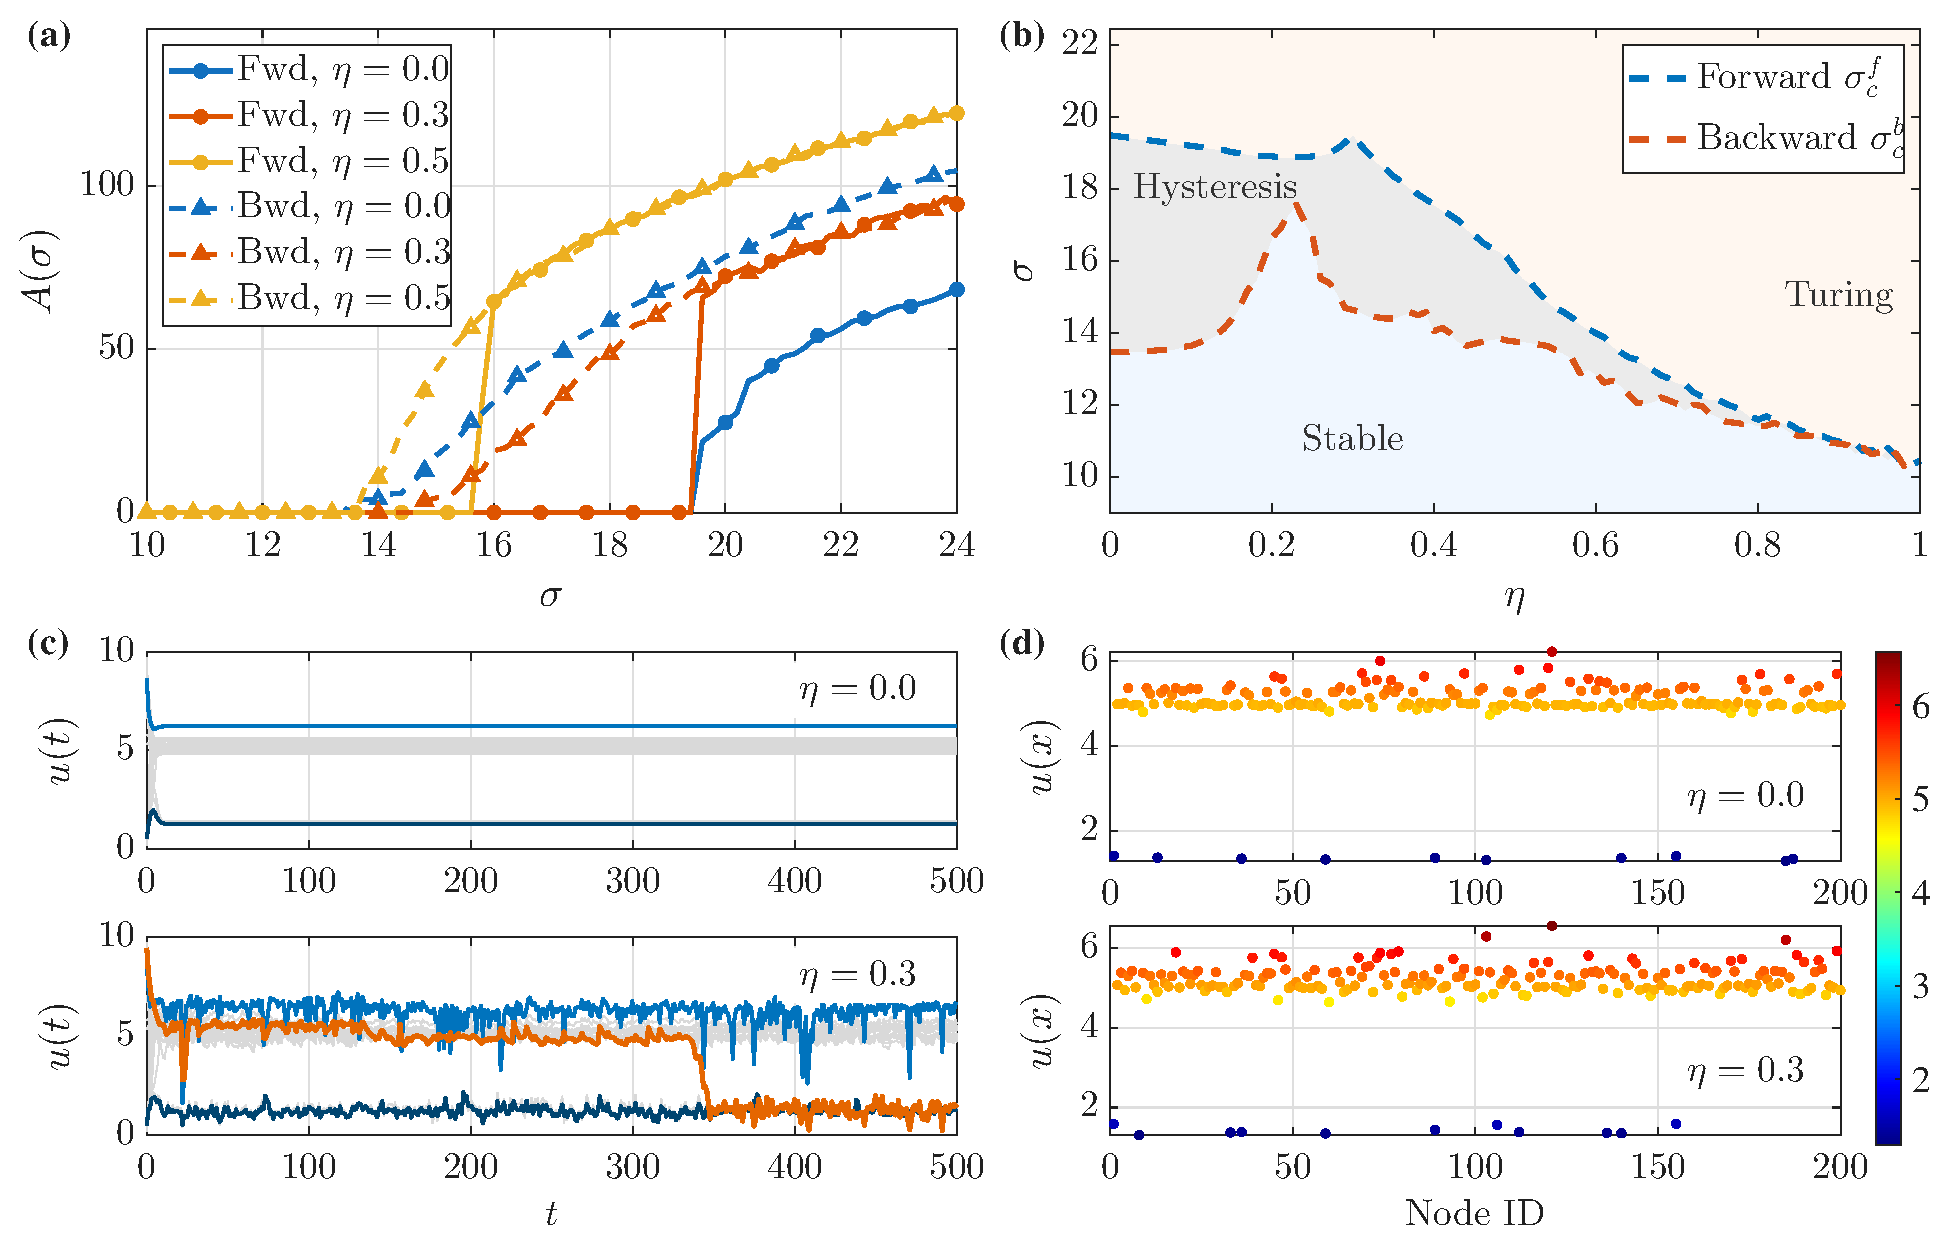
\includegraphics[width=\textwidth]{figures/fig1.eps}

	\caption{
		The multiplicative noise compresses the bistable region and facilitates pattern emergence.
		(a) The evolution of order parameter $A(\sigma)$ as the diffusion ratio $\sigma$ increases (forward, denoted Fwd) and decreases (backward, denoted Bwd) for different noise intensities, showing a clear hysteresis loop.
		(b) The phase diagram delineates the forward and backward critical values of $\sigma$ for varying noise intensities $\eta$, showing that the hysteresis region shrinks as $\eta$ increases and the multiplicative noise promotes the emergence of Turing patterns.
		(c) The temporal trajectories of the activator density $u$ within the first layer at $\eta = 0.0$ and $0.3$, where a noise-induced local transition occurs in a specific node, and the activator density drops from an activator-rich level near 5 to a depleted state near 0.
		(d) The corresponding stationary spatial distributions of $u$ across the first layer at $\eta = 0.0$ and $0.3$, further confirming that noise injects pronounced stochastic fluctuations into individual node dynamics while preserving the global self-organization.
	}
	\label{fig:noise}
\end{figure}

\subsection{Impact of noise}

The influence of noise on the system's global stability is characterized in \cref{fig:noise}.
In the deterministic limit ($\eta = 0$), the order parameter $A$ exhibits a discontinuous hysteresis loop as shown in \cref{fig:noise}(a), signifying a subcritical Turing bifurcation.
The system maintains bistability within the regime $\sigma \in (\sigma_c^b, \sigma_c^f)$, where the selection between the synchronized and pattern states depends on the initial conditions.

The introduction of multiplicative noise fundamentally reconstructs this stability landscape.
As depicted in \cref{fig:noise}(b), increasing noise intensity $\eta$ leads to a progressive contraction of the hysteresis region.
Specifically, the forward threshold $\sigma_c^f$ decreases monotonically, which indicates that noise-induced fluctuations disrupt the stability of the uniform state and facilitate an earlier transition to patterns.
Conversely, at low intensities, noise exerts a subtle stabilizing effect on the backward threshold $\sigma_c^b$.
Notably, as $\eta$ exceeds a critical level, the hysteresis loop vanishes entirely and the Turing transition evolves from a discontinuous jump to a smooth, supercritical bifurcation.

The temporal and spatial characteristics of these noise-driven dynamics are further detailed shown in \cref{fig:noise}(c-d).
The time evolution of node densities shown in \cref{fig:noise}(c) reveals a significant contrast: while the deterministic case ($\eta=0$) remains perfectly stable on the pattern branch, the introduction of multiplicative noise ($\eta=0.3$) triggers stochastic transitions of node states between the high- and low-density manifolds.
Despite these transitions, the spatial snapshots shown in \cref{fig:noise}(d) confirm that the system's macroscopic structure is preserved through a bimodal distribution.
This suggests that, while noise induces microscopic state-switching at the node level, the collective multiplex framework maintains a statistical integrity.

\subsection{Impact of multiplex structure}

\begin{figure}[!tb]
	\centering
	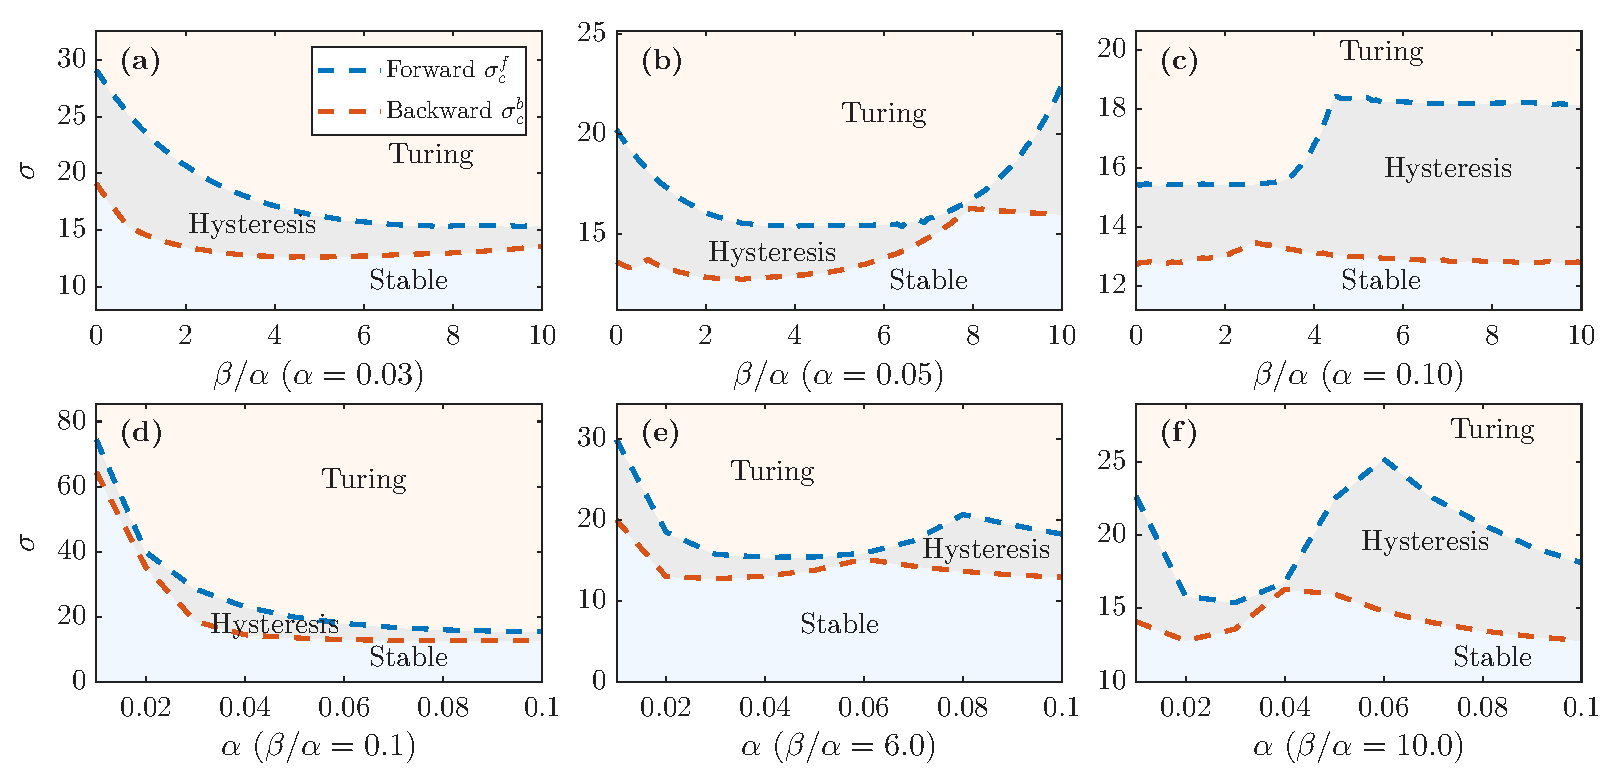
\includegraphics[width=\textwidth]{figures/fig2.eps}

	\caption{
		The multiplex network architecture exerts a complex non-monotonic influence on the Turing phase transitions and modulates the multistability region.
		(a)-(c) The phase diagrams delineating the forward critical boundary $\sigma_c^f$ and the backward critical boundary $\sigma_c^b$ against the inter-layer coupling $\beta/\alpha$ for fixed diffusion rates $\alpha$, demonstrating that a dominant inter-layer coupling effectively compresses the hysteresis loop at low $\alpha$ but substantially expands the bistable region at elevated $\alpha$.
		(d)-(f) The phase diagrams mapping the critical thresholds against the diffusion rates $\alpha$ under fixed inter-layer coupling $\beta/\alpha$, which show that a strong inter-layer coupling creates a distinct non-monotonic peak in the forward boundary at the intermediate diffusion levels and significantly broadens the hysteresis region.
	}
	\label{fig:multiplex}
\end{figure}

In the following, we investigate the collective impact of the diffusion coefficient $\alpha$ and the inter-layer coupling ratio $\beta/\alpha$ on the system stability.
As illustrated in \cref{fig:multiplex}(a), for a relatively low diffusion coefficient ($\alpha = 0.03$), both the forward and backward critical thresholds ($\sigma_c^f, \sigma_c^b$) decrease monotonically with $\beta/\alpha$, and the hysteresis loop gradually shrinks.
This suggests that, at this regime, inter-layer coupling acts as a facilitator for the emergence of Turing patterns.
However, a qualitative transition occurs as the internal diffusion increases.
For $\alpha = 0.05$ and $0.10$ (Figs. 2(b-c)), the critical points exhibit a non-monotonic dependence on the coupling ratio.
Specifically, the thresholds rise with $\beta/\alpha$, indicating that strong inter-layer coupling can suppress pattern formation at higher internal diffusion levels, before eventually reaching a saturation plateau at large $\beta/\alpha$.
This dual role of inter-layer coupling extends the results presented in \cite{Asllani2014PRE} and highlights the complex trade-off between individual layer instability and global multiplex synchronization.

The effect of $\alpha$ on the emergence of Turing patterns is shown in Figs. 2(d)-(f).
When the inter-layer coupling ratio is small ($\beta/\alpha = 0.1$), both $\sigma_c^f$ and $\sigma_c^b$ decrease rapidly as $\alpha$ increases and then stabilize at a low plateau.
This indicates that, for weakly coupled layers, the intra-layer diffusion $\alpha$ facilitates the onset of Turing patterns by lowering the required diffusion ratio $\sigma$.
However, as the inter-layer coupling becomes dominant ($\beta/\alpha = 1.0$ or $10.0$), a distinct non-monotonic behavior is observed.
While the backward threshold $\sigma_c^b$ remains relatively stable, the forward threshold $\sigma_c^f$ exhibits a prominent peak around $\alpha \approx 0.06$, leading to a significantly expanded bistable region.
The results shown in Figs. 2(d)-(f) clearly demonstrate that the presence of inter-layer coupling fundamentally alters the influence of diffusion on the Turing instability, creating a unique complexity that is absent in single-layer networks.

\subsection{Impact of intra-layer network topology}

\begin{figure}[!tb]
	\centering
	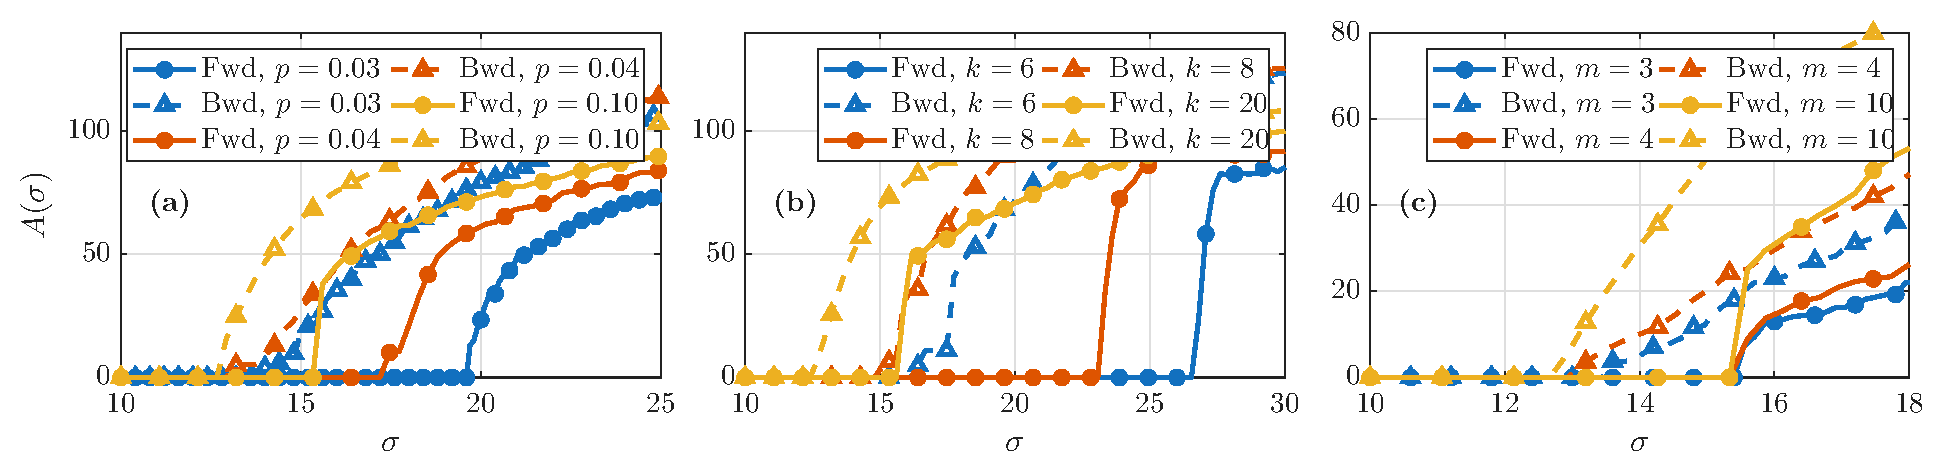
\includegraphics[width=\textwidth]{figures/fig3.eps}

	\caption{
		The evolution of the order parameter $A(\sigma)$ during forward and backward transitions across distinct complex networks, showing how network connectivity governs the sensitivity of Turing instability.
		(a) and (b) The amplitude profiles for ER and WS networks demonstrate a profound dependence on connectivity, confirming that increasing the connectivity (across $6$, $8$, and $20$) lowers the required diffusion thresholds.
		(c) The structural transitions on BA networks reveal a fundamentally different mechanism where structural heterogeneity dominates pattern onset, rendering the phase transitions insensitive to variations in connectivity.
	}
	\label{fig:topology}
\end{figure}

To evaluate the generality of our findings, we extend this investigation to WS small-world and BA scale-free topologies as shown in \cref{fig:topology}.
For homogeneous structures like ER and WS networks, a clear trend is observed from Figs. 3(a-b), where increasing the average degree $\langle k \rangle$ lowers both critical thresholds $\sigma_c^f$ and $\sigma_c^b$, while simultaneously compressing the hysteresis region.
This suggests that enhancing connectivity in these networks consistently facilitates the onset of Turing instability.

In contrast, the heterogeneous BA network exhibits a distinct behavior as shown in \cref{fig:topology}(c).
Remarkably, the forward critical point $\sigma_c^f$ remains virtually invariant regardless of the attachment parameter $m$.
This suggests that, in the scale-free architecture, the onset of pattern formation is primarily governed by the structural heterogeneity.
However, the backward threshold $\sigma_c^b$ still exhibits a downward shift with increasing $m$, and the order parameter $A$ grows more significantly in amplitude.
These results underscore that the intra-layer topology is a pivotal determinant of the Turing landscape.

\subsection{Impact of network size}

\begin{figure}[!tb]
	\centering
	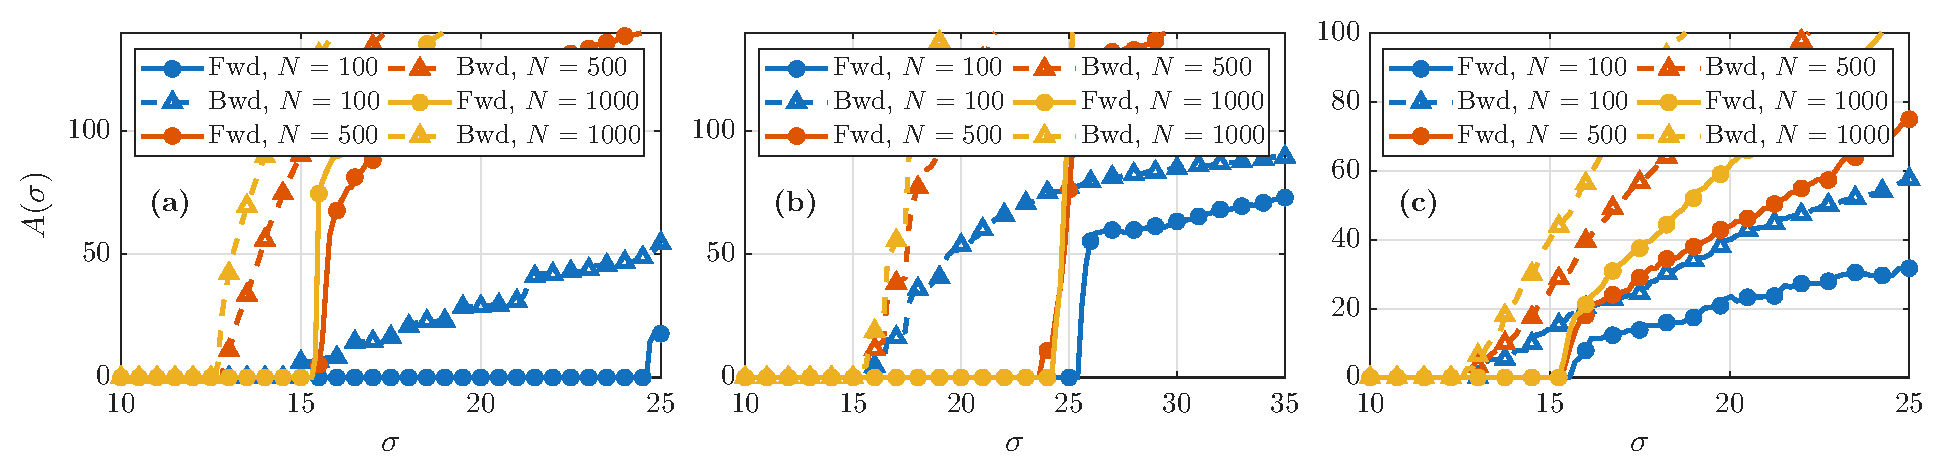
\includegraphics[width=\textwidth]{figures/fig4.eps}

	\caption{
		The evolution of the order parameter $A(\sigma)$ under varying network sizes $N$, demonstrating that the scale sensitivity of the Turing instability mirrors the previously observed connectivity effects.
		(a) and (b) The amplitude profiles for ER and WS networks exhibit a profound scale dependence, confirming that enlarging $N$ across 100, 500, and 1000 significantly accelerates pattern emergence.
		(c) The corresponding transitions on BA networks further validate the overarching dominance of the structural heterogeneity, rendering the critical phase boundaries remarkably robust and insensitive to the network scale.
	}
	\label{fig:size_impact}
\end{figure}

In the following, we investigate the influence of the network size $N$ on the hysteresis behavior as shwon in \cref{fig:size_impact}.
For the ER and WS networks (Figs. 4(a-b)), increasing $N$ from 100 to 1000 causes the forward critical threshold $\sigma_c^f$ to decrease, with the ER network exhibiting a more pronounced shift than the WS network.
In contrast, the forward threshold of the BA network (\cref{fig:size_impact}(c)) is remarkably insensitive to the system size and remains virtually constant. Despite these differences in the forward onset, the backward critical point $\sigma_c^b$ for all three topologies remains largely unaffected by $N$.
Furthermore, as the network scale expands, the order parameter $A$ is consistently enhanced, leading to a higher amplitude of the resulting Turing patterns across all network types.

\subsection{Impact of number of layers}

\begin{figure}[!tb]
	\centering
	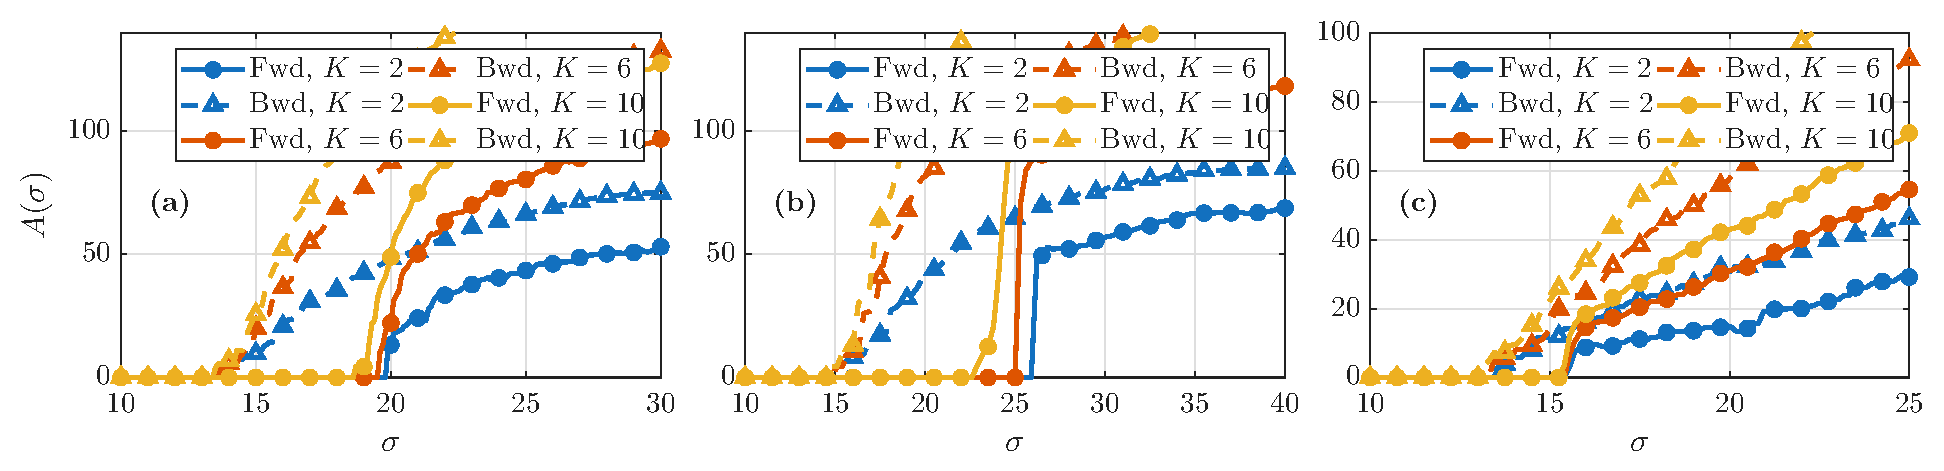
\includegraphics[width=\textwidth]{figures/fig5.eps}

	\caption{
		Extending the topological analysis to the multiplex dimension, the macroscopic transitions reveal how the number of layers $K$ modulates the diffusion thresholds across different architectures.
		(a) and (b) ER and WS networks maintain their structural vulnerability, where accumulating the layers across 2, 6, and 10 continuously lowers the required critical diffusion boundaries.
		(c) The pattern onset within BA networks proves that the structural heterogeneity completely overrides the multi-layer effect, guaranteeing that the hysteresis loops remain highly resilient and unaffected by variations of the layer count.
	}
	\label{fig:layer_impact}
\end{figure}

The influence of the number of layers $K$ on the hysteresis behavior is presented in \cref{fig:layer_impact}.
For both the ER and WS networks (Figs. 5(a-b)), an increase in $K$ from 2 to 10 causes a clear leftward shift in the forward critical thresholds $\sigma_c^f$.
This suggests that a higher degree of multiplexity in these relatively homogeneous topologies facilitates the emergence of Turing patterns.

In contrast, the BA network (\cref{fig:layer_impact}(c)) continues to demonstrate a unique robustness in its thresholds ($\sigma_c^f, \sigma_c^b$), which remains nearly invariant as $K$ increases.
While the onset point in the BA network is insensitive to the layer count, the amplitude of the order parameter $A$ is significantly bolstered.
This implies that, while the structural heterogeneity of the BA layers dictates the initiation of the instability, the additional layers provide a more extensive substrate that enhances the intensity of the resulting patterns.
Overall, these results indicate that increasing the number of network layers generally promotes instability and enhances pattern amplitudes, though the specific impact on the onset thresholds is mediated by the underlying intra-layer topology.

\section{Conclusion}\label{conclusion}

Recognizing that real-world populations and substances naturally disperse across interconnected layers, such as species migrating across multiple habitats, we constructed a multiplex-networked activator-inhibitor system model to capture these cross-layer interactions and diffusion processes.
Given that diffusive processes are inevitably subject to intrinsic fluctuations, we incorporated multiplicative noise into the model, thereby establishing a multiplex-networked stochastic reaction-diffusion system model.
In contrast to other studies that assume additive noise \cite{Karig2018,Asllani2013} or noise intensity tied to the difference from a homogeneous stationary state \cite{Xiao2023}, we considers the situation that the intensity of multiplicative noise is proportional to the local density differences between a node and its intra- and inter-layer neighbors, which more accurately aligns with realistic scenarios.

Analytically, by employing the stability theory of stochastic differential equations, we derived a sufficient condition for the almost sure asymptotic stability of the system.
The numerical simulations on the Mimura-Murray model revealed that multiplicative noise plays a profoundly constructive role in the emergence of Turing patterns.
Specifically, we demonstrated that such state-dependent fluctuations fundamentally alter the system's phase transitions by lowering the critical threshold for pattern onset and actively eliminating the subcritical hysteresis loop.

Furthermore, we systematically explored the impact of the multiplex architecture by varying the intra-layer diffusion coefficient and the inter-layer coupling strength.
While intra-layer diffusion generally promotes the emergence of Turing patterns, which aligns with the classical Turing mechanism, we demonstrated that inter-layer coupling exhibits a complex, non-monotonic influence.
Specifically, we show that, when intra-layer diffusion is weak, enhancing inter-layer coupling facilitates pattern formation, however, when diffusion dominates, increasing inter-layer coupling conversely suppresses the emergence of Turing patterns.
Furthermore,  we found that this suppression primarily elevates the forward critical threshold, which governs the transition from the synchronous state to the Turing pattern, while leaving the backward threshold largely unaffected.
This asymmetric effect significantly enlarges the hysteresis region.
Interestingly, the influence of inter-layer coupling is also subject to a saturation effect, such that once the coupling strength exceeds a certain level, the critical thresholds no longer exhibit significant variations.
Finally, from a topological perspective, we uncovered a striking scale-invariant robustness in BA networks.
We found that in such scale-free architectures, the threshold for the onset of Turing patterns is predominantly governed by the structural heterogeneity rather than the connectivity, the network size, and the number of layers.
This robust behavior contrasts sharply with the pronounced scale sensitivity observed generally from ER and WS networks.

Ultimately, our findings provide a deeper theoretical understanding of how the subtle interplay between multi-layer network topologies and stochastic fluctuations drives cross-layer pattern formation.
Future research could extend this framework to incorporate directed multiplex networks or time-varying topologies, bringing the mathematical modeling even closer to the dynamic realities of complex ecological and biological systems.

%%%%%%%%%%%%%%%%%%%%%%%%%%%%%%%%%%%%%%%%%%%%%%%%%%%%%%%
%%% Acknowledgements. 致谢
%%%%%%%%%%%%%%%%%%%%%%%%%%%%%%%%%%%%%%%%%%%%%%%%%%%%%%%
\Acknowledgements{
	% This work was supported by the National Natural Science Foundation of China (Grant Nos. 00000000 and 11111111).
	This work was supported by the National Natural Science Foundation of China (Grant No. 12271519),
	the Shenzhen Science and Technology Program (Grant No. JCYJ20240813101300001),
	the Fundamental Research Funds for the Central Universities (Grant Nos. 2023ZDYQ11005 and 2024KYJD2002),
	and the Hong Kong Research Grants Councile under GRF Grant CityU 11203725.
}

%%%%%%%%%%%%%%%%%%%%%%%%%%%%%%%%%%%%%%%%%%%%%%%%%%%%%%%
%%% Reference section. 参考文献
%%% Citation in the content using "some words~\cite{1,2}".
%%% ~ is needed to make the reference number is on the same line with the word before it.
%%% Using scis.bst to format the style if the ref.bib file is included, e.g.,
%%% \bibliographystyle{scis}
%%% \bibliography{ref}
%%%%%%%%%%%%%%%%%%%%%%%%%%%%%%%%%%%%%%%%%%%%%%%%%%%%%%%
\begin{thebibliography}{99}

	\bibitem{Cai2022}
	Cai R, Zhou H, Kou C. Active disturbance rejection control for fractional reaction-diffusion equations with spatially varying diffusivity and time delay. Sci China Inf Sci, 2022, 65: 129203

	\bibitem{Singh2026}
	Singh A K, Almsheks R, Kumar M, et al. The emergence of Turing instability and pattern formation in a nonlinear stochastic spatiotemporal epidemic model with reinfections. Acta Biotheor, 2026, 74: 10

	\bibitem{Ninomiya2024}
	Ninomiya H. Example of Turing's instability by equal diffusion. J Differ Equ, 2024, 392: 255

	\bibitem{Tompkins2014}
	Tompkins N, Li N, Girabawe C, et al. Testing Turing's theory of morphogenesis in chemical cells. Proc Natl Acad Sci USA, 2014, 111: 4397--4402

	\bibitem{Patti2023}
	Di Patti F, Biancalani T, Fanelli D. Stochastic Turing patterns in the Brusselator model. Phys Rev E, 2023, 107: 014201

	\bibitem{Liu2013}
	Liu Q-X, Doelman A, Rottsch\"afer V, et al. Phase separation explains a new class of self-organized spatial patterns in ecological systems. Proc Natl Acad Sci USA, 2013, 110: 11905--11910

	\bibitem{Giunta2020}
	Giunta G, Seyed-Allaei S, Gerland U. Cross-diffusion induced patterns for a single-step enzymatic reaction. Commun Phys, 2020, 3: 167

	\bibitem{Turing1952}
	Turing A. The chemical basis of morphogenesis. Phil Trans R Soc Lond B, 1952, 237: 37--72

	\bibitem{Gierer1972}
	Gierer A, Meinhardt H. A theory of biological pattern formation. Kybernetik, 1972, 12: 30--39

	\bibitem{Pigani2022}
	Pigani E, Sgarbossa D, Suweis S, et al. Delay effects on the stability of large ecosystems. Proc Natl Acad Sci USA, 2022, 119: e2203498119

	\bibitem{Grilli2017}
	Grilli J, Barab\`asi G, Michalska-Smith M J, et al. Higher-order interactions stabilize dynamics in competitive network models. Nature, 2017, 548: 210--213

	\bibitem{Sun2017}
	Sun Y-Z, Leng S-Y, Lai Y-C, et al. Closed-loop control of complex networks: a trade-off between time and energy. Phys Rev Lett, 2017, 119: 198301

	\bibitem{Jiang2023}
	Jiang S, Zhou J, Small M, et al. Searching for key cycles in a complex network. Phys Rev Lett, 2023, 130: 187402

	\bibitem{Qin2025}
	Qin B-W, Sheng W, Qian X, et al. Reordered hierarchical complexity in ecosystems with delayed interactions. PNAS Nexus, 2025, 4: pgaf214

	\bibitem{Yang2025}
	Yang Z, Wang L, Wang X, et al. Controllability of heterogeneous networked sampled-data systems. Sci China Inf Sci, 2025, 68: 132207

	\bibitem{Niu2026}
	Niu T, Mao B, Wang L, et al. Non-trivial consensus control on directed signed networks. Sci China Inf Sci, 2026, 69: 132203

	\bibitem{Sun2026}
	Sun Y, Wang H, Liu X, et al. Networked collective dynamics in animal ecology and cell biology. Phys Life Rev, 2026, 57: 4--60

	\bibitem{Othmer1971}
	Othmer H G, Scriven L E. Instability and dynamic pattern in cellular networks. J Theor Biol, 1971, 32: 507--537

	\bibitem{Othmer1974}
	Othmer H G, Scriven L E. Nonlinear aspects of dynamic pattern in cellular networks. J Theor Biol, 1974, 43: 83--112

	\bibitem{Horsthemke2004}
	Horsthemke W, Lam K, Moore P K. Network topology and Turing instability in small arrays of diffusively coupled reactors. Phys Lett A, 2004, 328: 444--451

	\bibitem{Moore2005}
	Moore P K, Horsthemke W. Localized patterns in homogeneous networks of diffusively coupled reactors. Physica D, 2005, 206: 121--144

	\bibitem{Gallos2004}
	Gallos L K, Argyrakis P. Absence of kinetic effects in reaction-diffusion processes in scale-free networks. Phys Rev E, 2004, 92: 138301

	\bibitem{Nakao2010}
	Nakao H, Mikhailov A S. Turing patterns in network-organized activator-inhibitor systems. Nat Phys, 2010, 6: 544--550

	\bibitem{Asllani2014}
	Asllani M, Challenger J D, Pavone F S, et al. The theory of pattern formation on directed networks. Nat Commun, 2014, 5: 4517

	\bibitem{Van2023}
	Van Der Kolk J, Garc\'ia-P\'erez G, Kouvaris N E, et al. Emergence of geometric Turing patterns in complex networks. Phys Rev X, 2023, 14: 021028

	\bibitem{Li2024}
	Li B, Zhu L. Turing instability analysis of a reaction-diffusion system for rumor propagation in continuous space and complex networks. Inf Process Manage, 2024, 61: 103621

	\bibitem{Zheng2023}
	Zheng Q, Shen J, Pandet V, et al. Turing instability in a network-organized epidemic model with delay. Chaos Solitons Fractals, 2023, 168: 113209

	\bibitem{He2023}
	He L, Su H. Turing pattern of an SIRI model on large-scale homogeneous and heterogeneous networks. Nonlinear Dyn, 2023, 111: 16605--16626

	\bibitem{Del2016}
	Del Genio C I, G\'omez-Garde\~nes J, Bonamassa I, et al. Synchronization in networks with multiple interaction layers. Sci Adv, 2016, 2: e1601679

	\bibitem{Shi2023}
	Shi L, Zhou J, Ye Y. Pattern formation in a predator-prey model with Allee effect and hyperbolic mortality on multiplex networks. Mathematics, 2023, 11: 3339

	\bibitem{Ye2025}
	Ye Y, Zhou J, Zhao Y. Pattern formation in reaction-diffusion information propagation model on multiplex simplicial complexes. Inf Sci, 2025, 689: 121445

	\bibitem{Zhao2025_PhysicaA}
	Zhao B, Shen J. Navigating epidemic spread through multiplex networks: Unveiling turing instability and cross-diffusion dynamics. Physica A, 2025, 660: 130312

	\bibitem{Fu2025}
	Fu S, Peng Q, He Y, et al. Unsupervised multiplex graph diffusion networks with multi-level canonical correlation analysis for multiplex graph representation learning. Sci China Inf Sci, 2025, 68: 132102

	\bibitem{Zhao2025_SCIS}
	Zhao T, Huang J, Wang Y, et al. Saturation function-based intermittent control on fixed-time output synchronization of multilayered networks. Sci China Inf Sci, 2025, 68: 209201

	\bibitem{Li2022}
	Li X, Li C, Li X. The impact of information dissemination on vaccination in multiplex networks. Sci China Inf Sci, 2022, 65: 172202

	\bibitem{Gong2024}
	Gong Y, Yang S, Liu S, et al. Strategies for mitigating detrimental effects in cyber-physical multiplex networks. Sci China Inf Sci, 2024, 67: 169201

	\bibitem{Asllani2014PRE}
	Asllani M, Busiello D M, Carletti T, et al. Turing patterns in multiplex networks. Phys Rev E, 2014, 90: 042814

	\bibitem{Asllani2013}
	Asllani M, Biancalani T, Fanelli D, et al. The linear noise approximation for reaction-diffusion systems on networks. Eur Phys J B, 2013, 86: 476

	\bibitem{Biancalani2017}
	Biancalani T, Jafarpour F, Goldenfeld N. Giant amplification of noise in fluctuation-induced pattern formation. Phys Rev Lett, 2017, 118: 018101

	\bibitem{Francesca2023}
	Francesca D P, Biancalani T, Fanelli D. Stochastic Turing patterns of trichomes in arabidopsis leaves. Proc Natl Acad Sci USA, 2023, 120: e2216368120

	\bibitem{Avitanile2026}
	Avitanile D, Maclaurin J. Neural fields and noise-induced patterns in neurons on large disordered networks. SIAM J Appl Math, 2026, 86: 427--456

	\bibitem{Butler2009}
	Butler T, Goldenfeld N. Robust ecological pattern formation induced by demographic noise. Phys Rev E, 2009, 80: 030902

	\bibitem{Butler2011}
	Butler T, Goldenfeld N. Fluctuation-driven Turing patterns. Phys Rev E, 2011, 84: 011112

	\bibitem{Biancalani2010}
	Biancalani T, Fanelli D, Di Patti F. Stochastic Turing patterns in the Brusselator model. Phys Rev E, 2010, 81: 046215

	\bibitem{Karig2018}
	Karig D, Martini K M, Weiss R, et al. Stochastic Turing patterns in a synthetic bacterial population. Proc Natl Acad Sci USA, 2018, 115: 6572--6577

	\bibitem{Xiao2023}
	Xiao R, Gao Q, Azaele S, et al. Effects of noise on the critical points of Turing instability in complex ecosystems. Phys Rev E, 2023, 108: 014407

	\bibitem{Barabasi1999}
	Barab\'asi A-L, Albert R. Emergence of scaling in random networks. Science, 1999, 286: 509--512

	\bibitem{Erdos1960}
	Erd\H{o}s P, R\'enyi A. On the evolution of random graphs. Publ Math Inst Hung Acad Sci, 1960, 5: 17--60

	\bibitem{Watts1998}
	Watts D J, Strogatz S H. Collective dynamics of `small-world' networks. Nature, 1998, 393: 440--442

	\bibitem{Sole2013}
	Sol\'e-Ribalta A, De Domenico M, G\'omez S, et al. Spectral properties of the Laplacian of multiplex networks. Phys Rev E, 2013, 88: 032807

\end{thebibliography}

\end{document}
